\chapter{Introduction}
\label{ch:introduction}

\gls{iot} is a relatively new concept that already has applications in many domains, creating new ways of interactions between humans and small devices, referred to as smart devices. \gls{iot} is being hailed as one of the primary catalysts of the next digital revolution. The technology enables connecting ubiquitous objects to the internet. The advancement of digital technologies, such as low-cost but highly capable sensors and processors, efficient wireless protocols, the mobile revolution, and a plethora of startups and established companies developing the necessary application and management software, are all contributing to the rise of IoT.
Applications like Smart Airports, Transportation, Home Automation, and more areas are being revolutionized by this technology \cite{marksteiner2017overview}.
\gls{iot} is the deployment of network-connected devices that interact with the physical environment by employing sensors to collect data, managing other systems, controlling actuators, as well as communicating with one another. Typically, an IoT solution's architecture incorporates constrained devices, gateways or border routers, and cloud-based services. Constrained devices are classified into three classes depending on their degree resources such as processing capability, memory, power supply, communication capability and user interfaces \cite{rfc7228}. Constrained devices may induce bottlenecks in the network and thus the network becomes a constrained network. However, constrained devices may also be operating in naturally constrained networks. Furthermore, depending on their class, they may be assumed to not be able to process sophisticated or even conventional cryptographic operations. In many use cases, the \gls{iot} devices handle critical and private data. This imposes the requirement for data integrity and authenticity guarantees, confidentiality of information, and privacy of users. Hence, the development in the field of \gls{iot} is challenging due to the nature of the limited environment.
\par
difficult topic not concenses adaptation is not directly possible
Security in IoT is still a hot topic as the direct adaptation of standard secure communication protocol solutions is confined. That is due to such solutions' expensive and resource-consuming operations, the constrained nature, and the scalability of IoT devices. For example \gls{tls} \cite{rfc5246}, which relies on \gls{tcp}, has been criticized as inappropriate for constrained \gls{iot} devices \cite{shang2016challenges}. Among the reasons are, the infeasibility of \gls{iot} devices to maintain long-lived connections due to energy constraints, high header overhead, and the low-latency requirement that is opposed by the delay due to \gls{tcp} handshake, especially in a lossy network. Nonetheless, research and development and continuously introducing functional alternatives. 
Alternatively, \gls{dtls} \cite{dtls} provides security for communication channels relying on \gls{udp}. In contrast to \gls{tcp}, \gls{udp} is more suitable for \gls{iot}. It is an unreliable protocol as it does not care about message delivery , resulting in a lower header overhead. In addition, it introduces less traffic to the network. On that basis, the \gls{ietf} introduced \gls{coap} \cite{rfc7252} that is intended to be a generic application protocol for constrained environments. Similar to the ubiquitous HTTP \cite{http}, \gls{coap} realizes a subset of the \gls{rest} architecture. Therefore, it easily translates to HTTP. Moreover, \gls{coap} leverages \gls{udp} as its transport layer protocol which is secured by \gls{dtls}. Hence, \gls{coap} is one of well-suited protocol alternatives for HTTP/TLS for \gls{iot}. Nevertheless, no single solution is perfect for all use cases as each has its own challenges and requirements.
\par
Security is an essential aspect of the different phases of the lifecycle of an IoT device. In addition to discussing the risks to a thing's security and the challenges that may be encountered in protecting against these threats, Garcia-Morchon et al. \cite{rfc8576} discuss the various stages in the lifecycle of a thing. The lifecycle of a thing is classified into four phases, as depicted in figure \ref{fig:iot-lifecycle}. In particular, our thesis is primarily focused on discussing the security of the bootstrapping phase and management of cryptographic keys during the operational phase to ensure desired security features for the utilized keys. Key management encapsulates the generation, exchange, storage, usage and replacement of cryptographic keys.
\begin{figure}[htbp]
	\centering
	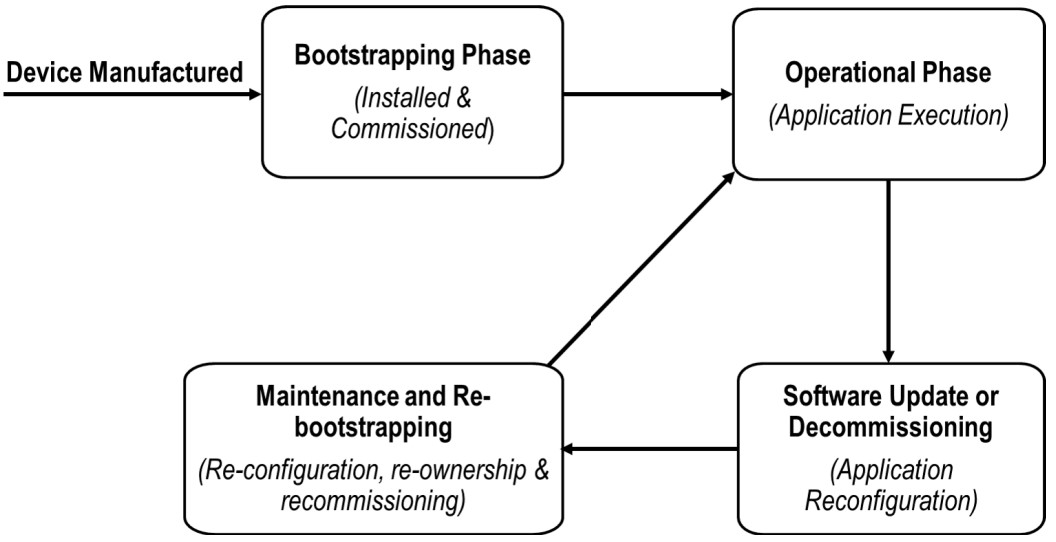
\includegraphics[scale=0.35]{Images/iot-lifecycle.jpg}
	\caption{Lifecycle of an \gls{iot} thing \cite{bs-survey}.}
	\label{fig:iot-lifecycle}
\end{figure}

\section{Research Aim and Contributions}\label{sec:reserach_questions}
The thesis aims to analyze and understand the relevance and importance of secure zero-touch bootstrapping and the future secrecy of cryptographic keys in IoT protocols. Furthermore, to present a proposal to implement future secrecy-related protocols in relevant use cases.
\par
The contributions of the thesis are the following:
\begin{itemize}
	\item We propose three use cases in which we discuss the applicability of the presented protocols.
	\item We conduct a comparative study between two secure bootstrapping protocols, \gls{brski} and \gls{sztp}.
	\item We give an overview over the \gls{x3dh} protocol and the double ratchet algorithm. In addition to present a formal verification of the \gls{x3dh} using \gls{ofmc}. Moreover, we discuss the post-quantum security of the protocols.
	\item We provide a demo implementation for \gls{x3dh} and the double ratchet algorithm using Python.
	\item We present a comparison between a set of certificate enrollment protocols in appendix \ref{appendix-enrollment}.
\end{itemize}

\section{Structure of the Thesis}\label{sec:structure_of_the_thesis}

The structure of this thesis is as follows: In chapter \ref{ch:background}, we reflect on principles relevant to the understanding of the work presented in further chapters. In addition to other works related to our thesis. 
Next we propose real-world use cases in chapter \ref{ch:usecases} where the protocols to be proposed can be applied.
In chapter \ref{ch:secureBootstrapping}, we give an overview of the two promising automated bootstrapping protocols: \gls{brski} and \gls{sztp}. Moreover, we present a comparative study between them.
Chapter \ref{ch:postcomp} discusses post-compromise security, and how it is achievable in an asynchronous environment through the use of \gls{x3dh} and double ratcheting. In addition, we discuss the formal verification of the protocols and their stand in the world of quantum computing.
In chapter \ref{ch:implementation} we present our demo implementation of the protocols discussed in chapter \ref{ch:secureBootstrapping}. 
Furthermore, chapter \ref{ch:discussion} discusses our findings and reflects the represented protocols on the use cases.
Finally, chapter \ref{ch:conclusion} concludes our work and introduces suggestions for future work.